\chapter[Anomaly Detection for the Roman Space Telescope Wide Field Instrument's Science Data Processing Pipeline]{Anomaly Detection for the Roman Space Telescope Wide Field Instrument's Science Data Processing Pipeline}
\label{ch:rst}
This chapter is from my published work \cite{horton2024anomaly} and builds off the work done in \cite{horton2020novelty} to develop a preliminary anomaly detection system for the Roman Space Telescope's Wide Field Instrument (WFI) Science Data Processing (SDP) pipeline.
This was a step away from the traditional image-based anomaly detection methods to a time series-based anomaly detection system by analyzing the up-the-ramp readout data from the WFI's H4RG-10 detectors instead of multispectral Mastcam images.
Because the new dimension added to the complexity of the data, I had to develop new methods for locating and classifying anomalies in the data, splitting the problem into two distinct tasks.
In addition to the original publication, a new section has been added to discuss the method used by the James Webb Space Telescope (JWST) for detecting cosmic rays. 
A full analysis of this method was not possible due to computational inefficiency, and is discussed as a future work.

\section{Abstract}
The Roman Space Telescope (RST) Wide Field Instrument (WFI) will be utilizing a preliminary Science Data Processing (SDP) pipeline during its Integration and Test, and potentially during Operations, to track basic statistics and identify known features such as cosmic rays, snowballs as well as possible anomalies in raw detector data. 
Snowballs are a newly recognized detector phenomenon that appear as circular clusters of pixels with large jumps in the ramp of a readout.
In our detectors, anomalies appear as jumps in the ramp of a readout and are classified as cosmic rays if they appear as a streak or snowballs if they're more circular. 
The WFI employs an array of 18 HgCdTe photodiode detectors (H4RG-10) that collect image samples.
Each set of raw frames within a non-destructive exposure is packaged by the SDP pipeline into image cubes for each detector.
Each cube is a time series of $4096 \times 4096$ accumulating pixel frames.
While snowballs are not fully understood, they are thought to be a feature of the detector itself through alpha decay of naturally radioactive contaminants.
The preliminary analysis pipeline is used to locate anomalies in these time-series accumulation frames and identify the type of anomaly, either natural phenomena or detector characteristics.
To compare different methods, we have implemented both heuristic-based and data-driven methods to identify anomalies.
For the heuristic-based approach, we identify snowballs and cosmic rays by the measured size and shape of outlier pixel clusters between consecutive frames.
For data-driven methods, we evaluated a Convolutional Neural Network (CNN) model and more traditional methods like Principal Component Analysis (PCA).
CNN is a supervised learning/classification method. 
Thus, we used a labeled dataset of anomalies to perform segmentation of the image and identify anomalies. 
We used previously identified cosmic rays and snowballs to measure the accuracy and efficiency of the mentioned approaches. 
In evaluating these methods, we aim to pick the best fit for the SDP pipeline's anomaly detection in terms of both performance and runtime. 

\section{Introduction}
The Roman Space Telescope (RST) Wide Field Instrument (WFI) employs an array of 18 H4RG-10 detectors to collect image sample \parencite{Mosby_2020}.
Each detector on the WFI utilizes an up-the-ramp readout scheme that produces $4096 \times 4096$ pixel images at each frame along the exposure. 
For a given exposure, each frame gives us information on the amount of light collected over time and allows us to identify both the location and time of anomalies within a ramp.
During an exposure, external or detector-related events may occur that affect groups (or sets) of pixels across the detector. 
External events, such as cosmic rays, involve something external to the detector causing a sudden increase in the amount of charge collected by the pixels.
Detector-related events, such as snowballs, are inherent to the detector and not caused by external sources.
While snowballs are not fully understood, their frequency and reoccurring locality lead us to believe they are a feature of the detector itself.
It is speculated that their origin may be due to alpha decay of naturally radioactive contaminants in the detector \parencite{cillis2018snowballs}.
Because we're collecting time-series information, we can see the exact frame in which the event occurs and observe how the event affects subsequent frames. 
There are many different sources that might cause errors in our detectors' data, such as read noise patterns, thermal noise, compression errors, and software errors, but we are particularly interested in external and natural sources of errors \parencite{cillis2018snowballs}. 
During Integration and Testing (I\&T) of the WFI detectors, identifying these errors is crucial to understanding the performance of the detectors and ensuring that they are functioning correctly before launch.
Understanding these errors ensures we select the best detectors for the WFI array and correctly identify issues with the detectors during operations.
Both cosmic rays and snowballs are transient events that result in sudden increases in charges and pixels' Data Number (DN) values compared to their typical neighboring pixels.
These events are also rare and not expected to occur in every exposure.
Therefore, we can use anomaly detection to identify these outliers as tracking the frequency of these events can help us identify issues with the detectors and their performance over time.
Figure \ref{rst/fig:anomalies} shows examples of these two events.

\begin{figure}
    \centering
    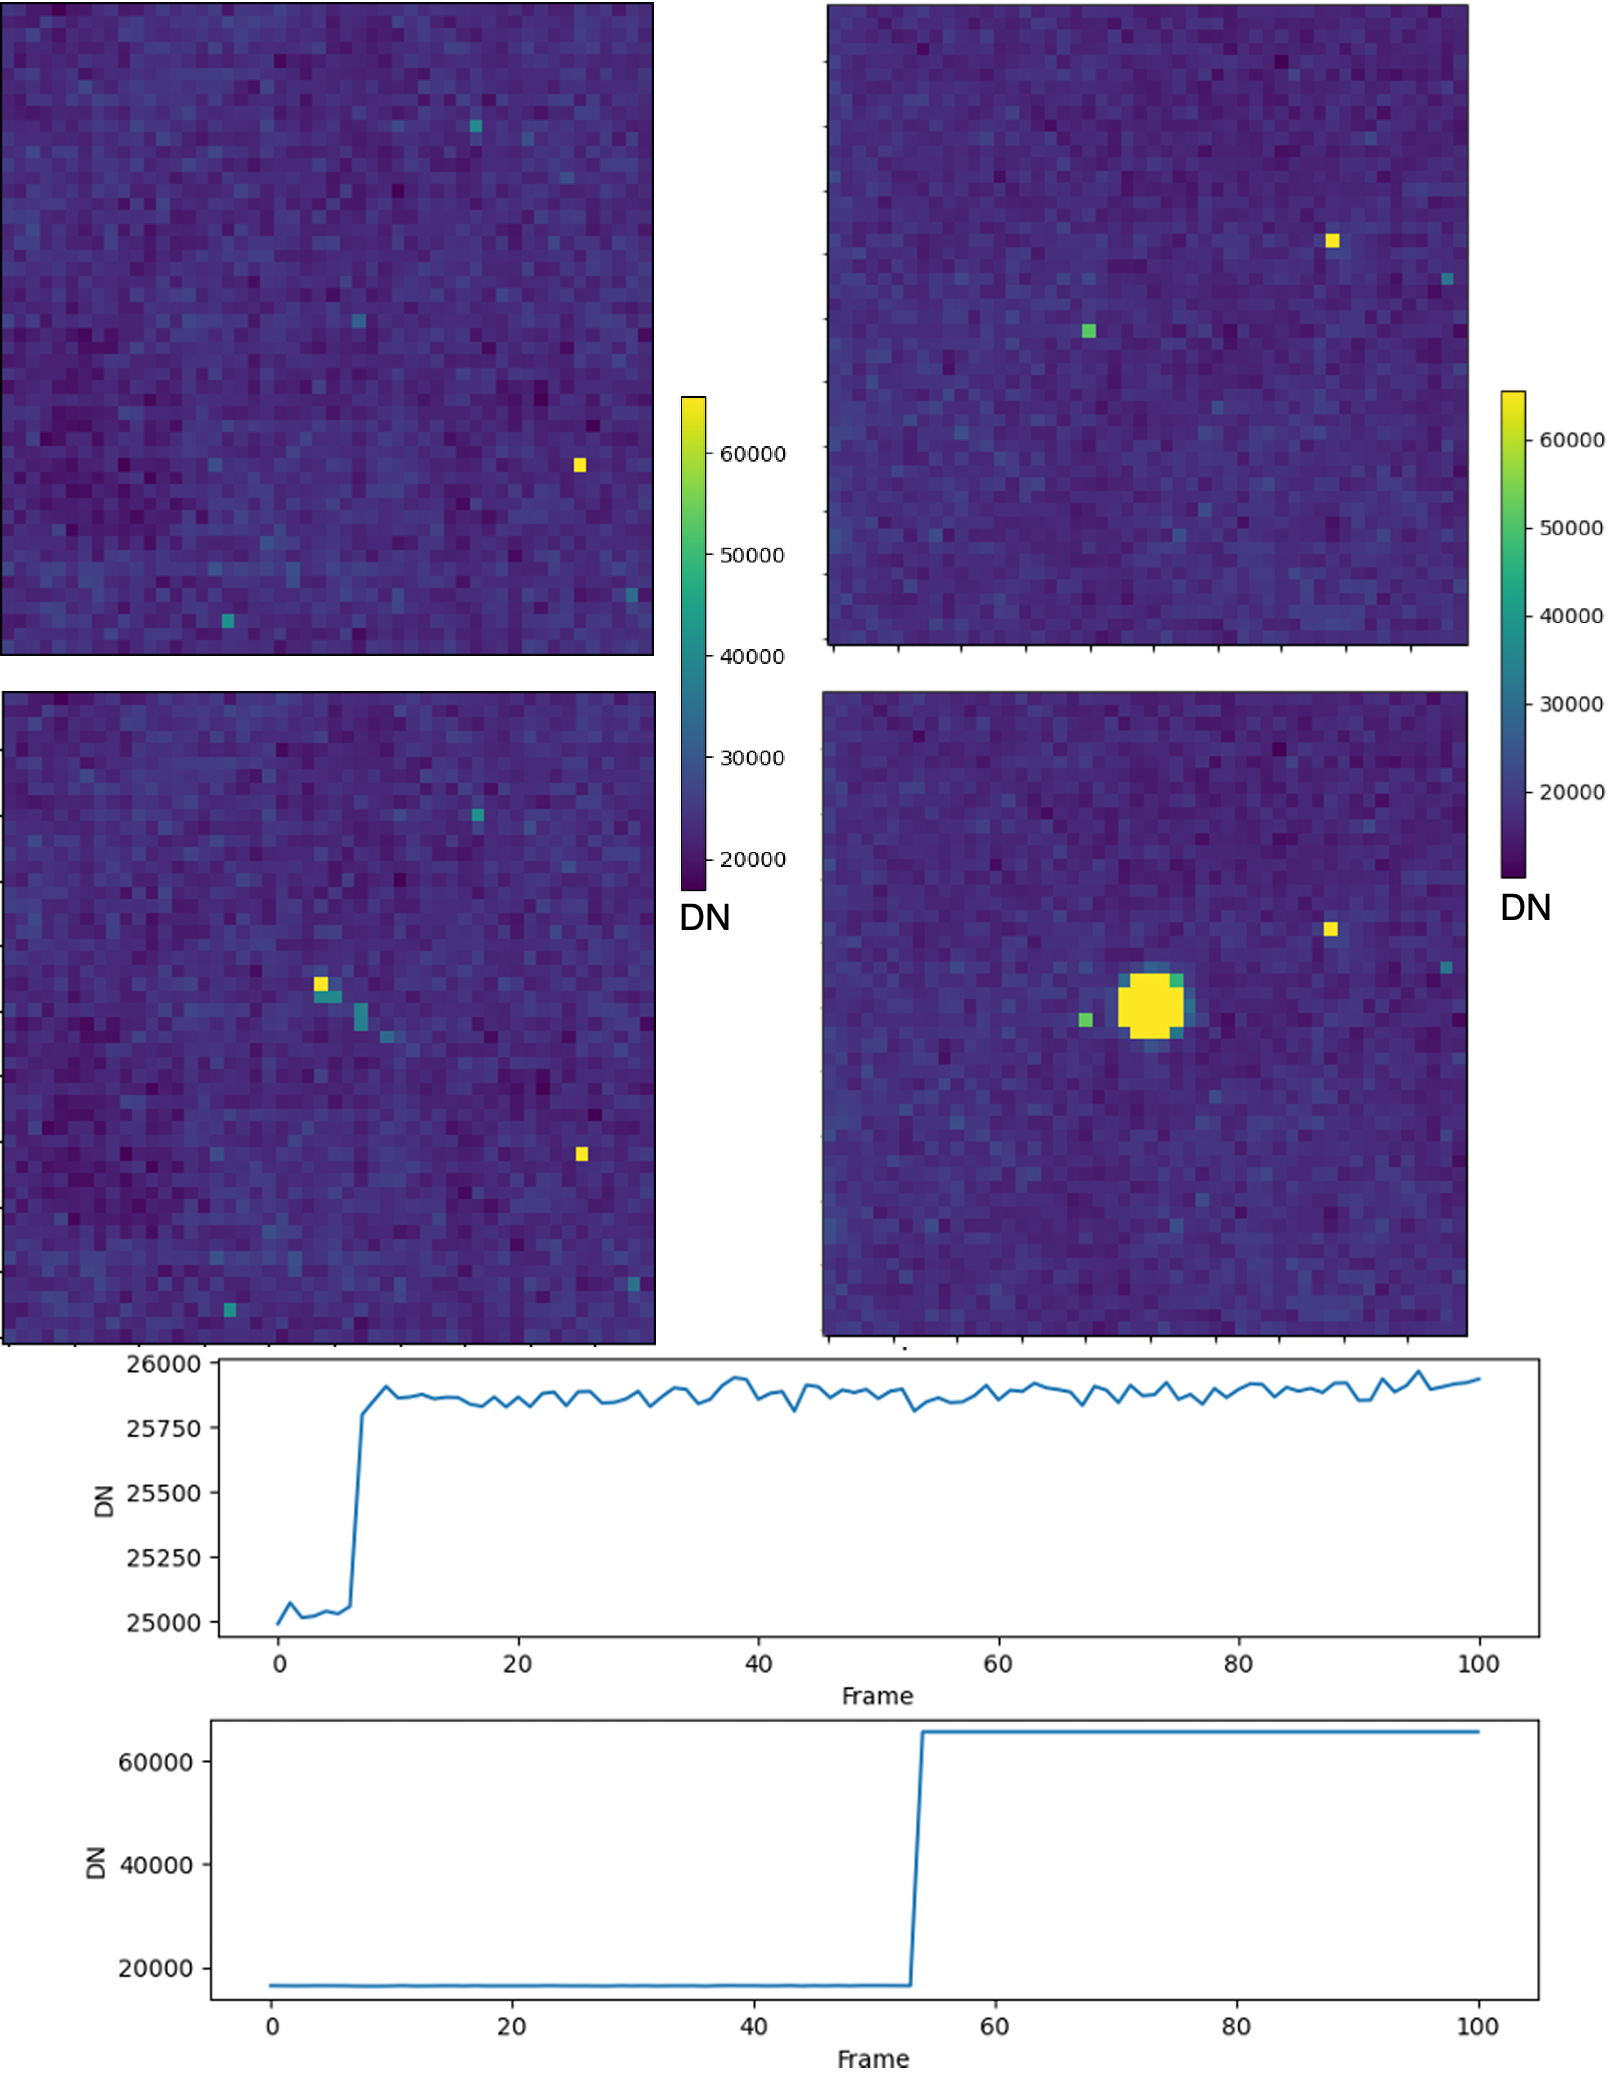
\includegraphics[width=.75\linewidth]{figs/rst/Examples_fixed.png}
    \caption[An Example of a Cosmic Ray and a Snowball in WFI Detector Data]{An example of a cosmic ray (left) and snowball (right) in RST's detector data. The top frames show the frame prior to the event, and the bottom frames show the area after the event has occurred. The bottom graphs show the overall DN value across the entirety of the exposure, showing large jumps at the time of the event for the cosmic ray (top) and snowball (bottom).}
    \label{rst/fig:anomalies}
\end{figure}

An anomaly is defined as an unexpected occurrence in a sequence based on a data set of typical sequences \parencite{horton2021integrating}. 
Given that our image is mostly typical pixels, we can use this feature to identify pixels that may be caused by snowballs or cosmic rays that are out of distribution. 
While snowballs are a newly recognized detector phenomenon, detection and rejection of anomalies are common practices for astronomical images \parencite{van2001cosmic}.
These cosmic rays appear as streaks across multiple pixels within an exposure as the incident cosmic ray imparts energy as a point spread function across neighboring pixels \parencite{pych2003fast}.

Both snowballs and cosmic rays will appear as jumps in DN value in a ramp but the shape of the affected neighboring pixels helps us differentiate between the two.
Snowballs will be circular in shape and affect nine or more pixels \parencite{cillis2018snowballs}.
On the other hand, cosmic rays will be any grouping larger than 2 pixels that shows a linear streak. 

The goal of our anomaly detection is to highlight these features as part of the RST WFI SDP's pipeline. 
As such, SDP's processing time should keep up with data generation time so that we can identify issues within the detectors as we collect new data. 
This poses a challenge due to the massive data size of the data products from the array of 18 detectors. 
To address this challenge, raw data is automatically processed into interpretable products as part of the SDP pipeline. 
As this anomaly detection system will be part of the SDP pipeline as an additional data product, the runtime of any method must be taken into account along with the method's accuracy. 

The rest of this chapter is organized as follows.
First, we go over the methods for identifying and classifying snowballs and cosmic rays in Section \ref{rst/sec:methods}.
Then, in Section \ref{rst/sec:data}, we explain the dataset chosen and how labels for the dataset were generated.
After that, we discuss the results of the different methods and draw conclusions about which methods to implement in the SDP pipeline in Section \ref{rst/sec:results}.
Section \ref{rst/sec:conclusions} concludes the work in this chapter.
Finally, we discuss future work in Section \ref{rst/sec:future}.

\section{Methods}
\label{rst/sec:methods}
To identify the anomalies in our data, we split our problem into two distinct subsequent tasks: 1) locating and grouping pixels that have irregular ramps and 2) classifying those pixels as cosmic rays, snowballs, or something else entirely.
We can use the first step to identify regions of interest and reduce our search area for snowballs and cosmic rays to that of anomalous pixels.
This can drastically reduce the number of pixels we have to classify as we also identify the frame in which the anomaly occurred, reducing our focus to a smaller window around the event. 
Table \ref{rst/tab:methods} list the methods used to accomlish locating and classifying anomalies.
Apart from the listed methods, there are other viable methods for accomplishing these tasks, such as Reed-Xiaoli (RX) and Localized Reed-Xiaoli (LRX) that are not implemented in this work.
RX is an unsupervised learning method that uses a window around a test pixel to compare with the local background \parencite{reed1990adaptive}.
LRX is similar to RX but instead uses a double concentric window to compare the test pixel with a guarded local background \parencite{molero2013analysis}.
Regardless of the method selected, the data must be loaded and preprocessed.
For more information about this and the dataset selection, see Section \ref{rst/sec:data}.

\begin{table}
    \centering
    \begin{tabular}{|l|l|}
            \hline
        \textbf{Step 1: Locating Anomalies} & \textbf{Step 2: Classifying Anomalies} \\
                \hline
        & Heuristic Rules \\
        Statistical Thresholding& \parencite{cillis2018snowballs} \\
        \hline
        Principal Component Analysis (PCA) & Convolutional Neural Network (CNN)\\
        \parencite{cillis2018snowballs} & \parencite{gu2018recent} \\
        \hline
        Generalized Least Squares (GLS) & \\
        \parencite{robberto2015cr} & \\
        \hline
    \end{tabular}
    \caption{Methods for Locating and Classifying Anomalies}
    \label{rst/tab:methods}
\end{table}


\begin{figure}[b]
    \centering
    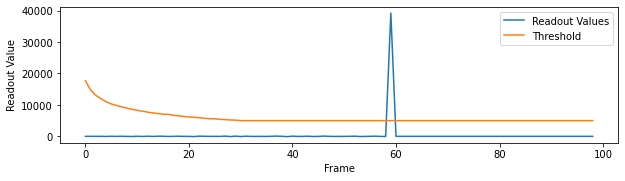
\includegraphics[width=1\linewidth]{figs/rst/Threshold.png}
    \caption[Readout Values Throughout a WFI Detector's Integration]{The readout values for a flagged pixel. The readout values are the amount of DN gained in a given frame. We compare this value to our calculated threshold, and if it is surpassed, that specific location and frame are flagged for classification.}
    \label{rst/fig:threshold}
\end{figure}
\subsection{Locating Anomalies}
To locate the anomalies, we looked for methods that would be able to not only identify where a potential anomaly is located but also when the event that caused the anomaly occurred. 
\subsubsection{Statistical Thresholding}
Our initial approach is readout thresholding, where we take two subsequent frames, $x_i$ and $x_{(i-1)}$ where $i$ is the frame number within an exposure of $n$ frames.
For each readout frame $\Delta x_i$, we calculate the mean $\mu_i$ and standard deviation $\sigma_i$ across its pixels. 
We use these values to calculate the threshold for jumps in the ramp with a minimum threshold value of 5000 DNs, as shown in Equation \ref{rst/equation:threshold}.
\begin{equation}
    \label{rst/equation:threshold}
    \Delta x_i > \max(\mu_i + 50 \sigma_i, 5000)
\end{equation}
These values were chosen for dark frames as they allow us to easily identify large jumps traditionally associated with snowballs or cosmic rays. 
From here, we create a pixel mask for each frame of all readout values that exceed this threshold. 
An example of a ramp from a single flagged pixel is shown in Figure \ref{rst/fig:threshold}.
We then perform a series of topological transformations to bridge and fill in incomplete holes through dilation, binary hole fill, and erosion procedures using SciPy's \texttt{ndimage} library \parencite{2020SciPy-NMeth}.
Finally, we remove any grouping of pixels of two pixels or less to ensure any jumps in the ramp we discover affect multiple pixels and then use scikit-image's \texttt{measure} library to locate the central pixel for each group \parencite{scikit-image}.
We are then left with groupings of pixels that could potentially be either a cosmic ray or a snowball or fall into the category of potential anomalies where the ramp is not typical but does not fit the criteria for either cosmic rays or snowballs.

\subsubsection{Principal Component Analysis (PCA)}
Given the majority of pixels within our image are not affected by anomalies, we can use a random subset of pixels within an exposure and fit PCA to the ramps of these samples.
If we limit our principal components to two, we can create a fit for the majority of simple ramps. 
Using our PCA fit, we can reduce all of the pixels in our image to our latent space representation and then inverse transform them to compare the original and reconstructed result \parencite{wold1987principal}.
Examples of this are shown in Figure \ref{rst/fig:PCA}. 

\begin{figure}
    \centering
    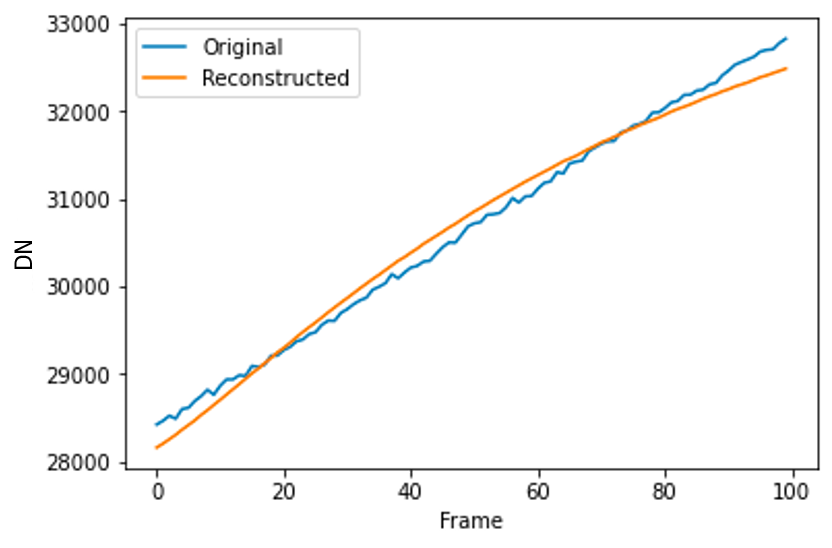
\includegraphics[width=0.49\linewidth]{figs/rst/PCA_Good.png}
    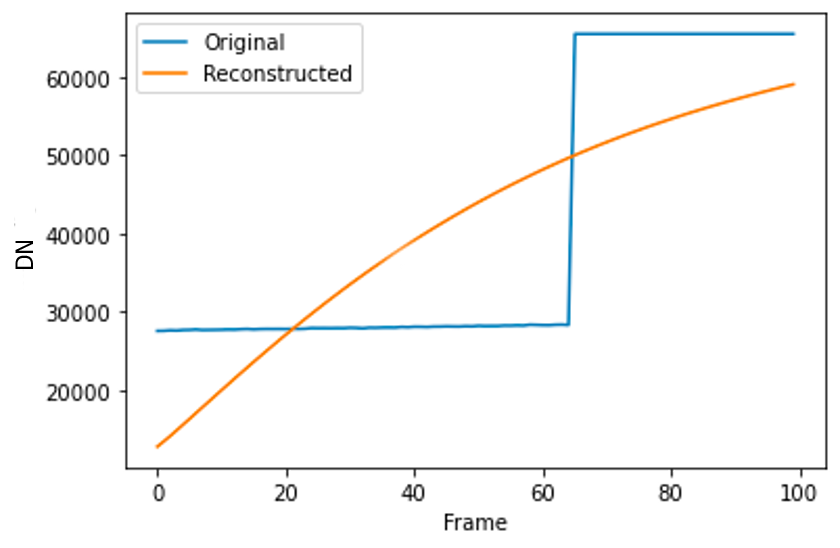
\includegraphics[width=0.49\linewidth]{figs/rst/PCA_Bad.png}
    \caption[Examples of using PCA to Ramp Jumps Through Reconstruction for WFI Detector Data]{Examples of reconstruction of ramps using PCA. The DN values for the reconstructed image are calculated by transforming the original values and then inverse-transforming our original ramp using only a subset of the principal components (i.e., two) to reproduce the shape. By limiting the number of principal components to two, we can have the reconstructed image fit the shape fairly well for normal ramps and not fit ramps with anomalies.}
    \label{rst/fig:PCA}
\end{figure}

With the reconstructed values, we are able to calculate the residual ($Image_{Reconstructed} - Image_{Original}$) of the errors and identify where anomalies occur based on spikes in the ramp of the residual. 
To identify these spikes, we can employ a method similar to the Statistical Threshold method to calculate the change in residuals between each frame and find out-of-distribution values. 
This results in identifying the frames for each pixel that have large jumps in the residual. 
By limiting the number of PCA components to two, our reconstructed ramps will be smooth, causing original ramps that have large jumps in them to have a large change in residual at the frame of the event.

Finally, like the statistical method, we create the pixel mask by highlighting any pixel whose change in residual is above the threshold.
We then identify regions using the same topological transformations and scikit-image's measure library for finding blobs \parencite{scikit-image}.

\subsubsection{Generalized Least Squares (GLS)}
JWST uses an GLS method, outlined in \cite{robberto2014generalized} to have a linear fit of non-destructive ramp by modeling the ramp of each pixel as well as the ramp if a jump were to occur at a given frame.
They then expanded their approach in \cite{robberto2015cr} to identify cosmic rays in their data in conjunction with Bayes factors to determine the likelihood of a cosmic ray occurring at a given frame, using a-prioi knowledge of the likelihood of cosmic rays occurring in a given exposure.
Using GLS over Ordinary Least Squares (OLS) is important because of three assumptions that OLS makes that GLS does not: the errors must be normally distributed, their variances must be consistent (points are spread around the regression line in the same way), and these errors must be uncorrelated. 
Having non-destructive frames with various sources of noise apart and anomalies violates the first two assumptions, making OLS not a good fit for our data.
In our case, we are interested in any jump in the ramp, regardless of the cause, so we can simplify the JWST method to just use the GLS method to produce metrics for each pixel and frame.

Using the Heaviside function, $\Theta(t)$, which returns 0 when less than 0 and 1 when greater than 0, we can fit a linear model of a ramp of $t_n$ values with a jump at a given frame $t_{CR}$ as follows:
\begin{equation}
    c(t_i) = a + b\ t_i + \text{CR}\ \Theta(t_i - t_{CR}) + \sigma_i
\end{equation}
In this equation, $a$ is the initial value of the ramp, $b$ is the slope of the ramp, $CR$ is the amount of DN added to the ramp at the time of the jump, and $\sigma_i$ is random error in the ramp.
In matrix form, this can be expressed as:
\begin{equation}
    c_i = \begin{bmatrix}
        c_1 \\
        c_2 \\
        \vdots \\
        c_n
    \end{bmatrix}
    A = \begin{bmatrix}
        1 & t_1 & 0 \\
        1 & t_2 & 0 \\
        \vdots & \vdots & \vdots \\
        1 & t_{CR} & 1 \\
        \vdots & \vdots & \vdots \\
        1 & t_n & 1
    \end{bmatrix}
    \alpha = \begin{bmatrix}
        a \\ b \\ \text{CR}
    \end{bmatrix}
\end{equation}
\begin{equation}
    \hat{c} = A \hat{\alpha}
\end{equation}
In order to test every possible frame for a jump, we can expand our matrix $A$ with a third dimension where each slice of the matrix is a different frame $t_{CR}$.
This results in a triangular matrix, with each column representing the possibility of a jump at that frame.
To solve for $\alpha$, we can use the GLS estimator \parencite{robberto2014generalized}:
\begin{equation}
    \hat{\alpha} = (\hat{A}^T W^{-1} \hat{A})^{-1} \hat{A}^T W^{-1} \hat{c}
\end{equation}
$W$ in our matrix is a covariance matrix that accounts for the noise in the data.
In the case of GLS, our covariance matrix is as follows:
\begin{equation}
    W = \begin{bmatrix}
        c_1 + \sigma_{ron}^2 & c_1 & \cdots & c_1 \\
        c_1 & c_2 + \sigma_{ron}^2 & \cdots & c_2 \\
        \vdots & \vdots & \ddots & \vdots \\
        c_1 & c_2 & \cdots & c_n + \sigma_{ron}^2
\end{bmatrix}
\end{equation}
where $\sigma_{ron}$ is the readout noise of the detector.
We can calculate the readout noise from the standard deviation of the readout values across a sample of pixels in the exposure.
Our matrix $\hat{A}$ is now three-dimensional, with shape (N, N, 3) to account for the jump occurring at each frame.
This will result in a two-dimensional matrix of $\hat{\alpha}$ values with shape (N, 3), where each slice of the row is the estimated parameters for a jump at that frame.
By calculating this all at once, we can quickly determine the residuals of each fit and identify the best fit for each pixel using matrix operations.

\subsection{Classifying Anomalies}
The other half of our implementation is classifying the anomalies we have located in the previous step.
We obtain a frame and pixel mask matrix containing information about potential anomalies with a ramp for each pixel in an exposure from the locating anomalies step.
We also obtain a table listing groupings of pixels to classify, known as the Event Table as it describes the time and location of potential anomalies. 
These groupings are the input into our classification methods as they help limit the search to specific pixels and frames across the exposure. 

\subsubsection{Heuristic Rules}
For Heuristic Rules, these groupings are labeled and measured by the number of pixels affected and the major and minor axes lengths of the affected area. 
We use these values to determine the type of anomaly.
Snowballs are large circular anomalies that cover nine or more pixels.
Cosmic rays are oblong anomalies that cover more than 2 pixels. 
We determine the circularity of the anomaly by comparing the minor and major axis using the following criteria.
\begin{align*}
    \text{Circular:}\ &  \text{minor\_axis} \geq \text{major\_axis}/2 \\
    \text{Large:}\ & \text{area} \geq 9
\end{align*}

From this, we are able to produce two output products: a new data cube where each frame is a mask identifying pixels affected by anomalies and an updated Event Table with information about each anomaly. 

\subsubsection{Convolutional Neural Network}
\label{rst/sec:CNN}
For each listing in the Event Table, we take a 32 square pixel sample region around the central pixel spatially and the three frames around the event frame for a sample of $32 \times 32  \times 3$ pixels. 
This is the input into our CNN, which is trained using hand-labeled data from the DCL dataset. 
The CNN architecture processes input images through two convolutional layers followed by ReLU activations and max pooling, which flattens the output.
Finally, we pass the output through two fully connected layers to produce class scores for None, Cosmic Rays, Snowballs, and Potential Anomalies classes based on the labeled dataset.
We performed two tests with the CNN by training and testing on all of the labeled datasets and just the data from the same detector to see how well the method generalizes. 
Both tests were performed with an 80/20 test/train split with balanced classes. 
The output classes from the CNN are then used to label the pixels in the mask with their associated class and update the Event Table with anomaly labels. 
\subsection{Output Products}
To align with the rest of the products from the SDP pipeline, we package the outputs from the anomaly detection pipeline as Hierarchical Data Format 5 (HDF5) files \parencite{The_HDF_Group_Hierarchical_Data_Format}.
HDF5 is a file format that is designed to store large amounts of data and is ideal for the types of products we need to produce for the SDP.
Because of HDF5's efficient read/write procedures, the SDP is able to keep up with the data generation rate while producing analysis products. 
For each exposure, we produce three binary mask arrays for events labeled as Cosmic Rays, Snowballs, and Potential Anomalies for each pixel within a ramp. 
These binary masks are the same shape as the exposure and enabling the ability to quickly identify and flag problem pixel/frame combinations in an exposure. 
We also produce a single quicklook summary image for each anomaly type, where each pixel is the frame number of an event. 
This allows us to visualize anomalies and see how they may change throughout an exposure.
Finally, the Event Table is formatted so that each row in the HDF5 array is an anomaly that has a central pixel, size, shape (semi-major and semi-minor axis), and classification as columns. 
These products are produced during the SDP pipeline and added as part of the automated report. 

\section{Data}
\label{rst/sec:data}
The H4RG detectors used in the WFI array are able to perform non-destructive reads while producing an exposure resulting in measurements through time, also referred to as up-the-ramp measurements. 
Non-destructive read means that the detector is able to read the pixel values without resetting them, allowing us to take multiple measurements of the same pixel during an exposure.
These individual reads accumulate throughout the exposure, resulting in a series of readout frames gradually increasing in DN value as the detector collects more light.
This allows us to take the up-the-ramp measurements taken during an exposure and order them in a series to create frames within the exposure. 
The result is a time series of frames for each integration from a detector's pixel values being reset at the beginning of an exposure to the final accumulated pixel values at the end of an exposure \parencite{casertano2022determining}.
To test the effectiveness of the anomaly detection pipeline, we use real exposures taken during the selection phase of the flight detectors for the WFI detector array. 
During the selection phase of flight detectors, over 70 detectors went through numerous experiments with different types of light exposures, both bright and dark.
These dark tests consisted of two-hour-long exposures where detectors accumulated across 100 frames.
We use these tests for identifying cosmic rays and snowballs due to their long exposure time, resulting in more opportunities for anomalies to appear in the frames. 
For the purposes of testing these methods, this chapter focuses on using only these dark exposures. 

The data from these tests are provided in the form of Flexible Image Transport System (FITS) files that consist of 101 frames of $4096 \times 4096$ pixel images \parencite{wells1979fits}.
The first frame in an exposure is the reset frame and can be disregarded. 
The FITS data is loaded into a NumPy array of unsigned integers by iterating over the array \parencite{harris2020array}.
To correct the read direction of FITS data, the data is processed by subtracting every pixel's value from the maximum possible DN value for each pixel, $2^{16} - 1$, across all frames.
This results in a data cube of $100$ frames, each with $4096 \times 4096$ pixels. 

The data provided by the Detector Characterization Lab (DCL) contains labeled information about known snowballs during the exposure. 
The DCL is responsible for characterizing the performance of the WFI detectors and identifying known issues with the detectors as well as selecting the best detectors for the WFI array \parencite{Mosby_2020}.
These snowballs are our preliminary ground truth for identifying the effectiveness of our methods. 
In addition to these snowballs, the outputs for each method are reviewed to identify snowballs and cosmic rays that are not in the original labels.
Because the heuristic method is overly sensitive, each anomaly highlighted by the method was hand-labeled as a potential anomaly, cosmic ray, snowball, or non-anomaly. 
These hand labels are used to measure the accuracy of each method and train methods such as the CNN in Section \ref{rst/sec:CNN}.

\section{Results}
\label{rst/sec:results}

As we are able to split our system into two different subsystems, the results here will discuss which of the methods are best for accomplishing each individual task. 
Then, we will go into more depth regarding the best method of integration pairing into the RST WFI SDP. 
For consistency, all of the tests were performed on a 2021 M1 Macbook Pro Max with 64GB of unified memory.
Much of the development of this work was done on the NASA Center for Climate Simulation PRISM GPU cluster. 

\subsection{Locating Anomalies}
The methods we tested for locating anomalies were Statistical Thresholding, PCA, and GLS.
These methods look for large jumps in a time series, but each method looks for a different type of jump.
The Statistical Thresholding method purely looks for jumps in the DN accumulated in each frame by identifying large changes in DN compared to the rest of the accumulated DN in the frame. 
The PCA method trains on a subset of pixels across the exposure and looks for large jumps in the residual error from transforming and inverse-transforming each pixel. 
Finally, the GLS method looks to fit a jump using a split linear fit across each frame.
Regarding runtime efficiency, all three methods require calculating the difference between values and a threshold and then identifying groups of flagged pixels. 
Statistical Thresholding only requires calculating the difference between two frames, while PCA requires calculating the difference between the original and reconstructed ramp.
On average, this takes about 2 minutes and 10 seconds for each dark image with 100 frames. 
Because PCA additionally needs to fit, transform, and inverse transform the entire exposure, running it adds an average of 42 seconds to locate anomalies. 
Finally, the GLS method takes over an hour just to calculate the residuals for each pixel across each frame.
This makes the statistical threshold method faster than PCA in every experiment because PCA requires preprocessing. 
GLS is far too slow to be considered for analysis without further optimization.

\begin{figure}
    \centering
    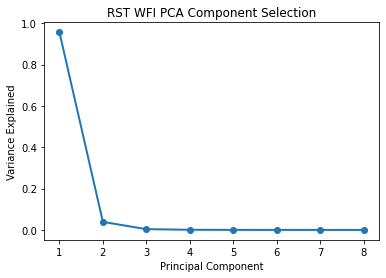
\includegraphics[width=.5\linewidth]{figs/rst/elbow.png}
    \caption[Elbow Plot of PCA for Typical Ramps in WFI Detector Data]{Elbow plot for the PCA method on typical ramps. A limit of 2 components was selected to ensure we aren't overfitting the curve and missing anomalies.}
    \label{rst/fig:elbow}
\end{figure}

As for accuracy, both PCA and Statistical Thresholding are over-sensitive to false positives.
The PCA method found fewer groupings than the Statistical Thresholding method, but many of the omitted groupings are false negatives.
Two principal components were chosen for PCA as additional components would result in overfitting to curves with jumps in the ramp.
Two components gives an overall shape that matches a typical ramp and explains most of the variance of the exposure's ramps without overfitting to the curve, as shown in Figure \ref{rst/fig:elbow}.
This false negative rate varies from exposure to exposure but ranges from 65 to 80\% missed anomalies. 
Despite being overly sensitive to any jump in the ramp, the Statistical Thresholding method is preferred here due to its higher accuracy and lower runtime.
Statistical Thresholding had a false negative rate of 10\% across the entire labeled dataset of over 5000 hand-labeled events. 
Statistical Thresholding filters most of the image without removing real anomalies is preferable to PCA which filters more of the images, including anomalies. 
The second step, Classifying Anomalies, can then label these false positives as None or Potential Anomalies. 

\subsection{Classifying Anomalies}
For classifying anomalies, we have the traditional method using Heuristic Rules around the shape of the grouping and the data driven CNN method trained on samples from the labeled anomalies. 
We utilized the output of the Statistical Thresholding method as the input into both of the classification methods. 
Neither method was ideal at accomplishing the task, but the Heuristic Rules method outperformed CNN by a wide margin in both accuracy and runtime.

We experimented with the CNN by training it on a subset of events in the Events Table that were hand-labeled by humans and then tested it on a separate set of events. 
We trained using a subset of all exposures in the labeled dataset as well as only exposures from a specific detector.
In both cases, we were unable to have the CNN generalize to different exposures. 
Because of the class imbalance and hard to differentiate nature of the dataset, the CNN would misclassify cosmic rays as potential anomalies and almost never correctly identify them as cosmic rays unless the streak was large enough to differentiate. 
The CNN was able to correctly classify snowballs about 50\% of the time, labeling them as potential anomalies in other cases. 
In the future, this method may be better suited than Heuristic Rules, but further refining of the labeled dataset is necessary.
As it stands, with the overlap between cosmic rays and potential anomalies, there is little room for improvement without further defining how we want to differentiate these classes.

Heuristic Rules outperformed our CNN method in both accuracy and runtime.
Figure \ref{rst/fig:heuristic_confusion} shows the confusion matrix for the Heuristic Rules method with the located data from the Statistical Thresholding method.
This combination method was able to find every pre-labeled snowball from the original dataset and correctly identify 85 out of 137 (62\%) of hand-labeled snowballs. 
The outputs from the Event Table in locating anomalies include measurements of the size and shape of the anomaly. 
This makes it very efficient to run through each entry of the table and pre-define a look-up table to classify each anomaly. 
The time the Heuristic Rules pipeline takes to generate a report depends on the number of anomalies in the Event Table, but, on average, it is able to classify 100 events from the Event Table per second. 

\begin{figure}
    \centering
    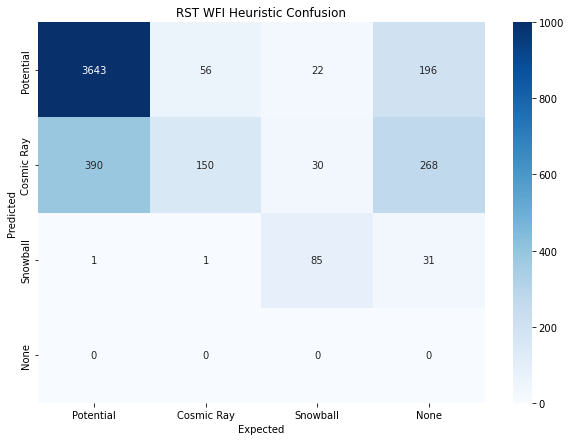
\includegraphics[width=.7\textwidth]{figs/rst/heuristic_confusion.png}
    \caption[Confusion Matrix for Heuristic Rules with Statistical Thresholding]{Confusion matrix for the Heuristic Rules method with located data from Statistical Thresholding.}
    \label{rst/fig:heuristic_confusion}
\end{figure}

\section{Conclusions}
\label{rst/sec:conclusions}
In this chapter, we have outlined the methods used to identify and classify anomalies in the RST WFI detector data.
We have shown that Statistical Thresholding is the best method for locating anomalies in the data, as it is able to identify the majority of anomalies while being fast enough to keep up with the data generation rate.
We have also shown that Heuristic Rules is the best method for classifying anomalies, as it is able to correctly identify the majority of snowballs and cosmic rays while being fast enough to keep up with the data generation rate.
Additionaly, we have tested other methods such as PCA and GLS, but these methods were either too slow or not accurate enough to be used in the SDP pipeline.

With further optimization, the GLS method may outperform PCA and Statistical Thresholding as it is designed to identify cosmic rays in a similar up-the-ramp readout scheme.
However, because linear regression is necessary across every pixel and every frame, the method is too computationally expensive to run on the entire exposure.
Even with numerical optimizations, such as avoiding the inverse matrix calculation using NumPy's Singular Value Decomposition based Least Squares algorithm, the GLS method is still too slow to be used in the SDP pipeline \parencite{harris2020array}.
Figure \ref{rst/fig:jwst_gls}, shows an example of the GLS method from two samples, with and without a snowball.
In the example with a snowball, GLS is able to identify both the jump in the ramp and the location of the jump.
Looking at the residuals, the massive dip in mean squared error at the time of the jump is due to the GLS method fitting perfectly to the ramp.
In the case without a snowball, almost every fit is perfect, as GLS was finding tiny jumps at each frame instead of the larger jumps we were looking for.

While this method works well for identifying a single pixel with a jump, it does not scale well once we take into consideration the number of pixels in an exposure.
The GLS method may produce a better metric than simple Statistical Thresholding to spot differences between two frames, but it is not efficient enough to run on the entire exposure.
If the GLS calculation could be optimized, such as only calculating the GLS for pixels that have been flagged by the Statistical Thresholding method, we may be able to use it in the future.

\begin{figure}
    \centering
    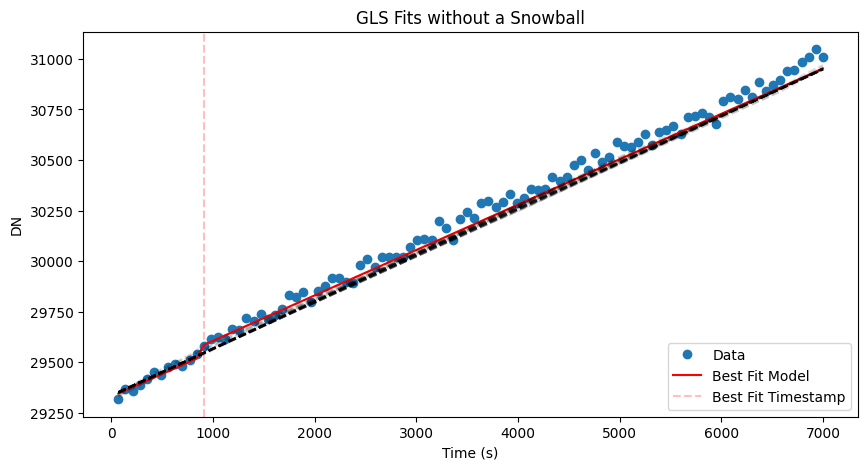
\includegraphics[width=.49\linewidth]{figs/rst/gls_good.png}
    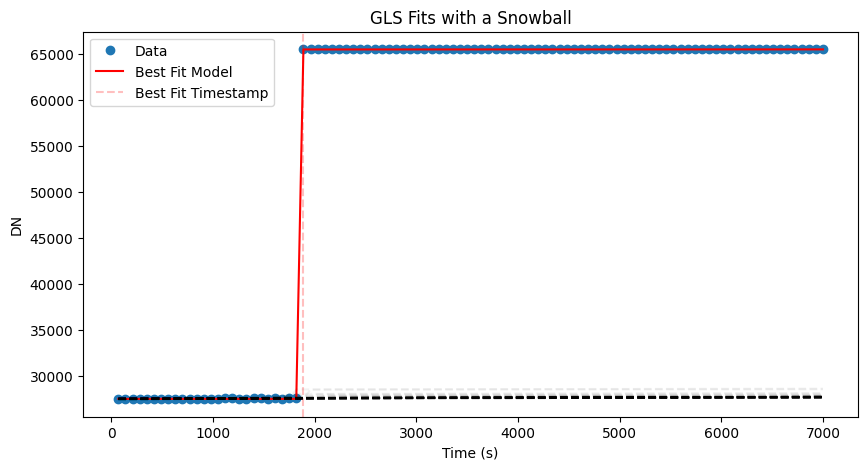
\includegraphics[width=.49\linewidth]{figs/rst/gls_bad.png}
    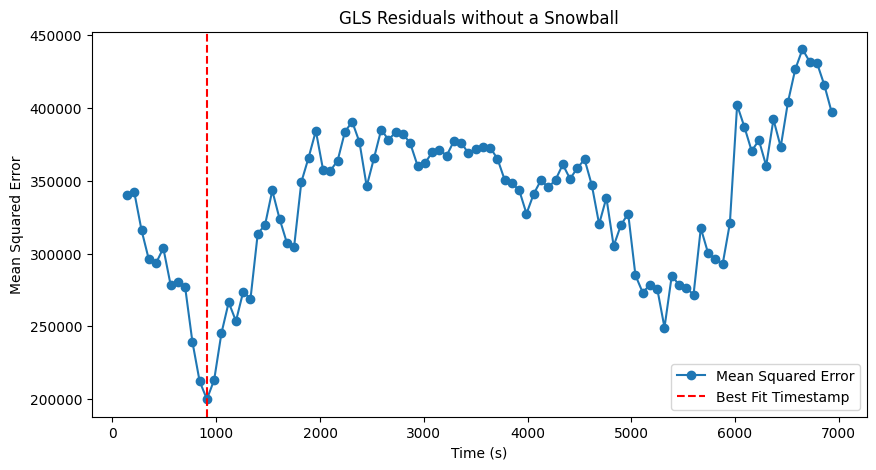
\includegraphics[width=.49\linewidth]{figs/rst/gls_good_res.png}
    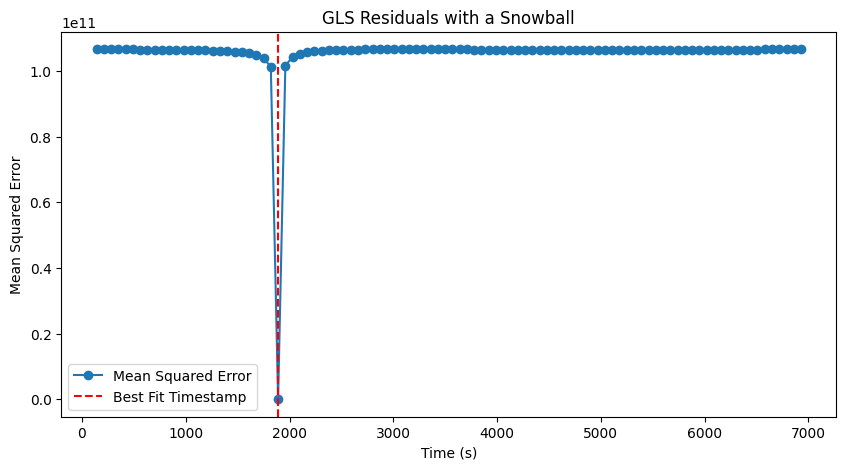
\includegraphics[width=.49\linewidth]{figs/rst/gls_bad_res.png}
    \caption[Example of the GLS Method on WFI Detector Data]{
        An example of the GLS method on WFI detector data.
        The two images on the left show a standard ramp with no anomalies, with the top showing how GLS fits the ramp and the bottom showing the mean squared error residuals of the fit.
        The two images on the right show a ramp with a snowball in the middle of the exposure, with the top showing how GLS fits the ramp and the bottom showing the mean squared error residuals of the fit.
        Note the scales on the residual plots are vastly different.
        In the case of the snowball, the GLS method only fits at one point in the ramp, resulting in a large dip in the residuals near that point and a large error at all other points.
    }
    \label{rst/fig:jwst_gls}
\end{figure}

\subsection{SDP Pipeline Integration}
Of the methods tested, the best combination of methods for the SDP pipeline would be the Statistical Thresholding method for locating anomalies and the Heuristic Rules method for classifying anomalies.
This combination is easy to implement in the SDP pipeline and is fast enough to keep up with the data generation rate of the WFI detectors.
This method is not without its flaws, as it produces many false positive cosmic rays that should be labeled as potential anomalies or None.
This is likely due to the less rigid criteria for identifying cosmic rays compared to snowballs.
Currently, this combination has been provided to the SDP team for integration into the pipeline as a library, following the same structure as the rest of the SDP pipeline.

\section{Future Work}
\label{rst/sec:future}
This work is a preliminary analysis of the anomaly detection methods for the RST WFI SDP pipeline.
There are many areas for improvement and future work to be done.
First and foremost, more methods will need to be evaluated in order to determine a better alternative to the Heuristic Rules method for classification. 
The CNN method is a good candidate but needs more fine-tuning to generalize to different exposures.
In addition to this, more labeled data will be needed to train the CNN and other methods, such as Mask RCNN or transformer-based architectures, particularly on illuminated data.
This labeled data could come from other exposures if we were to generalize beyond just the dark exposures.
With a well-defined dataset of labeled data, we will be able to better assess the accuracy of these methods, too. 

Another area for improvement may be finding better ways to locate anomalies.
We may revisit PCA to see if we can adjust the parameters (number of components and threshold for error) to reduce its false negative rate.
We may also revisit GLS if we can determine a way to optimize the algorithm further to make it viable for massive image sizes. 
Updating GLS to the full JWST method using Bayes factors may also help reduce the false positive rate of the method and provide a normalized metric for thresholding.
Additionally, other methods like RX and LRX, as described at the beginning of Section \ref{rst/sec:methods}, could be better suited for filtering the initial exposure.

The current implementation of the SDP pipeline uses a bad pixel mask to mask regions of the image that are problematic. 
Because we didn't have a bad pixel mask for the data we were using, we had to analyze the entire image with our anomaly detection methods.
This led to a large number of false positives from known bad pixels that appeared as anomalies in the dataset due to their sharp ramp in DN values at the beginning of the exposure.
In the future, we will need to integrate the bad pixel mask into the anomaly detection pipeline to filter out these false positives and use that to better assess the accuracy of the system. 

Finally, we will need to test the system on more than just dark exposures.
The current system is designed to work with dark exposures, but we will need to adjust the system to work with other types of exposures that might have more difficulty detecting anomalies.
There may not be a one-size-fits-all solution to this problem, but testing different types of exposures will help us determine the best methods for each type of exposure.